\section{Inverter test}
\label{app:inverter_step_test}
\subsection*{Purpose:}
The purpose of this test is to investigate the behavior of the inverter when applying a power step.  

\subsection*{Test equipment:}

\begin{itemize}
\item SMA STP20000 inverter
\item DEIF ASC controller 
\end{itemize}

\subsection*{Procedure:}

\textbf{Setup:}
%
\begin{itemize}
\item Connect the DC supply to the inverter 
\item Connect the inverter to the grid in parallel mode
\end{itemize}

The next step in this test is to run the test sequence. 
The inverter is only tested up to 50\% load as the available DC source is incapable of delivering more power to test further steps.
The test is conducted with different types of loads, real and reactive, where the reactive is tested with both capacitive and inductive loads.  

\textbf{Program:}
\begin{enumerate}
\item The ASC sends a power reference of 0 \% to the inverter by Modbus.
\item The ASC sends power references of 25\% or 50\% to the inverter by Modbus.
\item The ASC sends a power reference of 0 \% to the inverter by Modbus.
\item Repeat step 1 to 3 until both step sizes are tested for all load types. 
\end{enumerate}


\subsection*{Measuring data:}
The measuring data can be found on the CD under the path: \path{CD:/Measuring_data/Inverter_test_standalone}


\subsection*{Results:}
The plotted measuring data is shown in \figref{fig:inverter_data}, here the data is formatted to start at the same time so the different steps easily can be compared.

\begin{figure}[H]
\centering
% This file was created by matlab2tikz.

% The latest updates can be retrieved from
%  http://www.mathworks.com/matlabcentral/fileexchange/22022-matlab2tikz-matlab2tikz
% where you can also make suggestions and rate matlab2tikz.

\definecolor{mycolor1}{rgb}{0.00000,0.44700,0.74100}%
\definecolor{mycolor2}{rgb}{0.85000,0.32500,0.09800}%
\definecolor{mycolor3}{rgb}{0.92900,0.69400,0.12500}%
\definecolor{mycolor4}{rgb}{0.49400,0.18400,0.55600}%
\definecolor{mycolor5}{rgb}{0.46600,0.67400,0.18800}%
\definecolor{mycolor6}{rgb}{0.30100,0.74500,0.93300}%

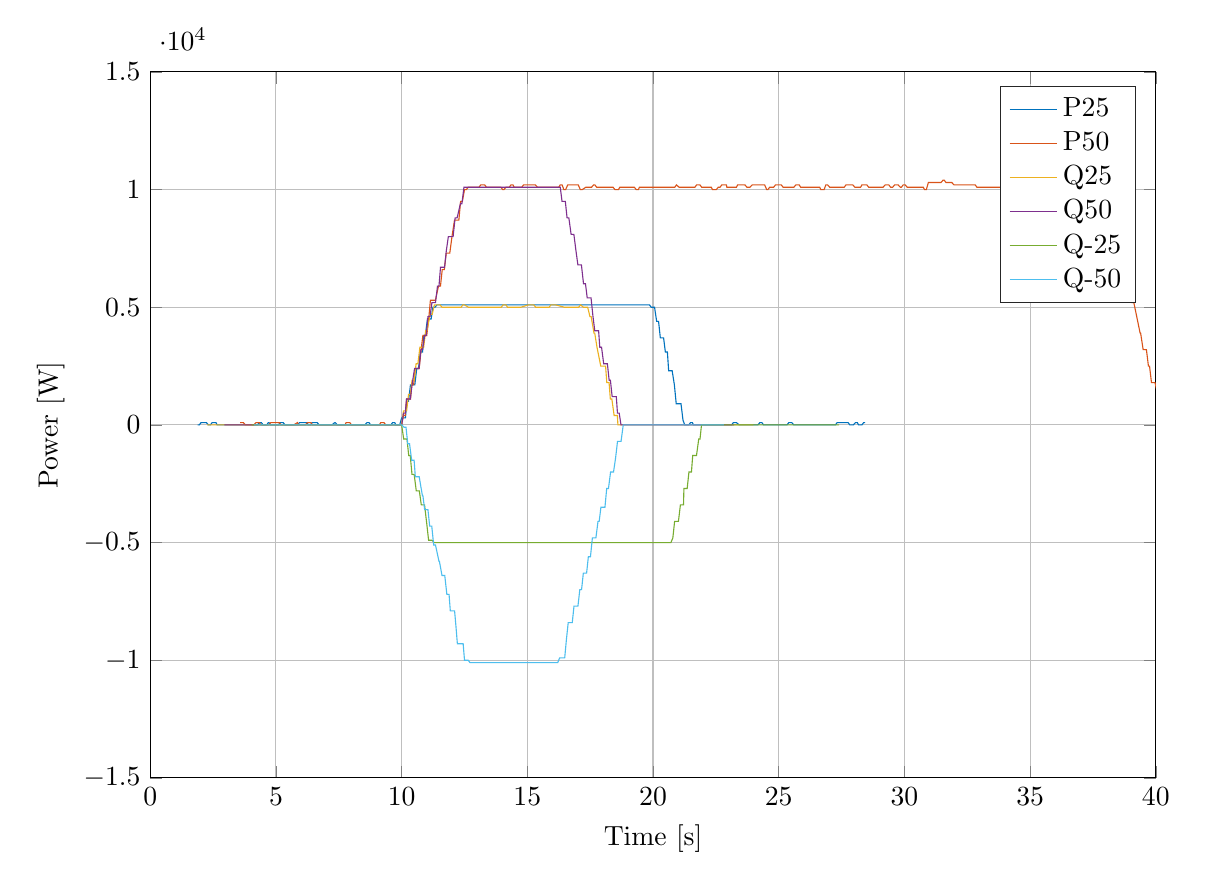
\begin{tikzpicture}

\begin{axis}[%
width=5.028in,
height=3.53in,
at={(1.85in,0.746in)},
scale only axis,
xmin=0,
xmax=40,
xlabel={Time [s]},
xmajorgrids,
ymin=-15000,
ymax=15000,
ylabel={Power [W]},
ymajorgrids,
axis background/.style={fill=white},
legend style={legend cell align=left,align=left,draw=white!15!black}
]
\addplot [color=mycolor1,solid]
 table[row sep=crcr]{%
1.882	0\\
1.952	0\\
2.022	100\\
2.102	100\\
2.162	100\\
2.232	100\\
2.318	0\\
2.393	0\\
2.463	100\\
2.532	100\\
2.616	100\\
2.663	0\\
2.733	0\\
2.816	0\\
2.893	0\\
2.964	0\\
3.033	0\\
3.083	0\\
3.163	0\\
3.233	0\\
3.317	0\\
3.394	0\\
3.464	0\\
3.535	0\\
3.585	0\\
3.665	0\\
3.735	0\\
3.82	0\\
3.865	0\\
3.935	0\\
4.055	0\\
4.075	0\\
4.145	0\\
4.195	0\\
4.266	0\\
4.336	100\\
4.419	100\\
4.495	0\\
4.636	0\\
4.696	100\\
4.722	100\\
4.796	0\\
4.876	0\\
4.956	0\\
5.006	0\\
5.096	0\\
5.166	100\\
5.236	100\\
5.286	100\\
5.367	0\\
5.437	0\\
5.521	0\\
5.597	0\\
5.677	0\\
5.721	0\\
5.797	0\\
5.868	0\\
5.937	100\\
6.019	100\\
6.097	100\\
6.167	100\\
6.238	100\\
6.288	0\\
6.368	0\\
6.438	100\\
6.522	100\\
6.578	100\\
6.639	100\\
6.725	0\\
6.799	0\\
6.869	0\\
6.939	0\\
7.021	0\\
7.07	0\\
7.14	0\\
7.225	0\\
7.34	100\\
7.36	100\\
7.44	0\\
7.49	0\\
7.57	0\\
7.65	0\\
7.7	0\\
7.77	0\\
7.823	0\\
7.9	0\\
7.97	0\\
8.04	0\\
8.123	0\\
8.2	0\\
8.27	0\\
8.324	0\\
8.4	0\\
8.47	0\\
8.54	0\\
8.623	100\\
8.7	100\\
8.77	0\\
8.84	0\\
8.922	0\\
9	0\\
9.07	0\\
9.14	0\\
9.223	0\\
9.27	0\\
9.34	0\\
9.423	0\\
9.5	0\\
9.571	0\\
9.641	100\\
9.724	100\\
9.771	0\\
9.841	0\\
9.923	0\\
10.001	300\\
10.071	300\\
10.151	300\\
10.211	1000\\
10.272	1000\\
10.351	1700\\
10.401	1700\\
10.471	1700\\
10.524	1700\\
10.602	2400\\
10.671	2400\\
10.742	3100\\
10.832	3100\\
10.882	3800\\
10.942	3800\\
11.025	4500\\
11.102	4500\\
11.173	4500\\
11.243	5000\\
11.326	5000\\
11.403	5100\\
11.472	5100\\
11.528	5100\\
11.603	5100\\
11.673	5100\\
11.726	5100\\
11.803	5100\\
11.932	5100\\
11.943	5100\\
12.029	5100\\
12.103	5100\\
12.173	5100\\
12.227	5100\\
12.304	5100\\
12.374	5100\\
12.444	5100\\
12.528	5100\\
12.604	5100\\
12.674	5100\\
12.728	5100\\
12.805	5100\\
12.875	5100\\
12.944	5100\\
13.027	5100\\
13.105	5100\\
13.175	5100\\
13.228	5100\\
13.305	5100\\
13.376	5100\\
13.429	5100\\
13.507	5100\\
13.577	5100\\
13.646	5100\\
13.729	5100\\
13.807	5100\\
13.877	5100\\
13.934	5100\\
14.008	5100\\
14.077	5100\\
14.147	5100\\
14.23	5100\\
14.307	5100\\
14.377	5100\\
14.431	5100\\
14.518	5100\\
14.578	5100\\
14.718	5100\\
14.732	5100\\
14.809	5100\\
14.879	5100\\
14.949	5100\\
15.034	5100\\
15.11	5100\\
15.179	5100\\
15.25	5100\\
15.332	5100\\
15.379	5100\\
15.449	5100\\
15.532	5100\\
15.609	5100\\
15.68	5100\\
15.75	5100\\
15.837	5100\\
15.881	5100\\
15.95	5100\\
16.034	5100\\
16.11	5100\\
16.181	5100\\
16.252	5100\\
16.302	5100\\
16.382	5100\\
16.452	5100\\
16.535	5100\\
16.582	5100\\
16.652	5100\\
16.735	5100\\
16.813	5100\\
16.893	5100\\
16.937	5100\\
17.013	5100\\
17.083	5100\\
17.153	5100\\
17.223	5100\\
17.323	5100\\
17.384	5100\\
17.455	5100\\
17.505	5100\\
17.575	5100\\
17.656	5100\\
17.738	5100\\
17.786	5100\\
17.856	5100\\
17.94	5100\\
18.027	5100\\
18.087	5100\\
18.157	5100\\
18.207	5100\\
18.278	5100\\
18.358	5100\\
18.441	5100\\
18.488	5100\\
18.558	5100\\
18.641	5100\\
18.718	5100\\
18.788	5100\\
18.858	5100\\
18.944	5100\\
18.989	5100\\
19.058	5100\\
19.142	5100\\
19.219	5100\\
19.289	5100\\
19.359	5100\\
19.444	5100\\
19.489	5100\\
19.559	5100\\
19.642	5100\\
19.719	5100\\
19.789	5100\\
19.859	5100\\
19.929	5000\\
19.99	5000\\
20.06	5000\\
20.144	4400\\
20.22	4400\\
20.29	3700\\
20.4	3700\\
20.42	3700\\
20.49	3100\\
20.571	3100\\
20.621	2300\\
20.691	2300\\
20.761	2300\\
20.849	1700\\
20.922	900\\
20.992	900\\
21.062	900\\
21.112	900\\
21.192	200\\
21.262	0\\
21.348	0\\
21.422	0\\
21.492	100\\
21.562	100\\
21.613	0\\
21.683	0\\
21.763	0\\
21.848	0\\
21.923	0\\
21.993	0\\
22.064	0\\
22.114	0\\
22.184	0\\
22.264	0\\
22.35	0\\
22.394	0\\
22.464	0\\
22.547	0\\
22.634	0\\
22.674	0\\
22.748	0\\
22.824	0\\
22.895	0\\
22.965	0\\
23.047	0\\
23.125	0\\
23.195	100\\
23.266	100\\
23.316	100\\
23.425	0\\
23.457	0\\
23.537	0\\
23.597	0\\
23.668	0\\
23.752	0\\
23.828	0\\
23.898	0\\
23.968	0\\
24.05	0\\
24.098	0\\
24.168	0\\
24.25	100\\
24.328	100\\
24.398	0\\
24.468	0\\
24.518	0\\
24.598	0\\
24.669	0\\
24.752	0\\
24.829	0\\
24.898	0\\
24.968	0\\
25.018	0\\
25.099	0\\
25.169	0\\
25.252	0\\
25.329	0\\
25.399	100\\
25.469	100\\
25.519	100\\
25.599	0\\
25.669	0\\
25.752	0\\
25.819	0\\
25.86	0\\
25.94	0\\
26	0\\
26.055	0\\
26.13	0\\
26.2	0\\
26.27	0\\
26.34	0\\
26.421	0\\
26.471	0\\
26.556	0\\
26.632	0\\
26.692	0\\
26.755	0\\
26.822	0\\
26.902	0\\
26.962	0\\
27.054	0\\
27.123	0\\
27.203	0\\
27.257	0\\
27.323	100\\
27.404	100\\
27.458	100\\
27.524	100\\
27.605	100\\
27.675	100\\
27.759	100\\
27.825	0\\
27.905	0\\
27.966	0\\
28.057	100\\
28.126	100\\
28.176	0\\
28.246	0\\
28.307	0\\
28.377	100\\
28.437	100\\
};
\addlegendentry{P25};

\addplot [color=mycolor2,solid]
 table[row sep=crcr]{%
3.573	100\\
3.634	100\\
3.704	100\\
3.785	0\\
3.874	0\\
3.934	0\\
4.005	0\\
4.055	0\\
4.126	0\\
4.205	100\\
4.289	100\\
4.336	100\\
4.406	0\\
4.489	0\\
4.566	0\\
4.636	0\\
4.706	0\\
4.796	100\\
4.846	100\\
4.906	100\\
4.989	100\\
5.066	100\\
5.136	100\\
5.206	0\\
5.294	0\\
5.337	0\\
5.407	0\\
5.49	0\\
5.567	0\\
5.637	0\\
5.707	0\\
5.857	100\\
5.892	0\\
5.957	0\\
6.007	0\\
6.09	0\\
6.167	0\\
6.257	100\\
6.307	100\\
6.39	100\\
6.457	0\\
6.527	0\\
6.598	0\\
6.678	0\\
6.738	0\\
6.808	0\\
6.891	0\\
6.968	0\\
7.038	0\\
7.093	0\\
7.168	0\\
7.238	0\\
7.308	0\\
7.392	0\\
7.458	0\\
7.548	0\\
7.638	0\\
7.658	0\\
7.748	0\\
7.792	100\\
7.868	100\\
7.938	100\\
8.008	0\\
8.092	0\\
8.168	0\\
8.238	0\\
8.291	0\\
8.369	0\\
8.439	0\\
8.509	0\\
8.591	0\\
8.669	0\\
8.739	0\\
8.792	0\\
8.869	0\\
8.94	0\\
9.01	0\\
9.111	0\\
9.17	100\\
9.211	100\\
9.294	100\\
9.372	0\\
9.452	0\\
9.496	0\\
9.572	0\\
9.653	0\\
9.696	0\\
9.773	0\\
9.843	0\\
9.914	0\\
9.997	0\\
10.074	400\\
10.144	400\\
10.197	1100\\
10.274	1100\\
10.355	1100\\
10.399	1700\\
10.475	1700\\
10.545	2400\\
10.615	2400\\
10.698	2400\\
10.776	3200\\
10.845	3800\\
10.915	3800\\
10.999	3800\\
11.076	4500\\
11.145	5300\\
11.199	5300\\
11.276	5300\\
11.345	5300\\
11.466	5900\\
11.475	5900\\
11.545	5900\\
11.615	6600\\
11.698	6600\\
11.775	7300\\
11.845	7300\\
11.915	7300\\
12.002	8000\\
12.103	8700\\
12.146	8700\\
12.199	8700\\
12.276	8700\\
12.346	9500\\
12.416	9500\\
12.501	10000\\
12.576	10000\\
12.646	10100\\
12.699	10100\\
12.776	10100\\
12.846	10100\\
12.917	10100\\
13	10100\\
13.077	10100\\
13.147	10200\\
13.217	10200\\
13.302	10200\\
13.377	10100\\
13.447	10100\\
13.517	10100\\
13.605	10100\\
13.647	10100\\
13.717	10100\\
13.803	10100\\
13.878	10100\\
13.948	10100\\
14.018	10000\\
14.068	10000\\
14.149	10100\\
14.202	10100\\
14.279	10100\\
14.349	10200\\
14.429	10200\\
14.479	10100\\
14.549	10100\\
14.619	10100\\
14.702	10100\\
14.78	10100\\
14.85	10200\\
14.92	10200\\
15.003	10200\\
15.15	10200\\
15.18	10200\\
15.251	10200\\
15.321	10200\\
15.403	10100\\
15.481	10100\\
15.541	10100\\
15.612	10100\\
15.692	10100\\
15.752	10100\\
15.821	10100\\
15.904	10100\\
15.982	10100\\
16.052	10100\\
16.104	10100\\
16.182	10100\\
16.252	10100\\
16.306	10200\\
16.383	10200\\
16.453	10000\\
16.524	10000\\
16.606	10200\\
16.683	10200\\
16.754	10200\\
16.808	10200\\
16.884	10200\\
16.955	10200\\
17.025	10200\\
17.108	10000\\
17.185	10000\\
17.325	10100\\
17.345	10100\\
17.413	10100\\
17.486	10100\\
17.555	10100\\
17.636	10200\\
17.686	10200\\
17.756	10100\\
17.826	10100\\
17.91	10100\\
17.986	10100\\
18.066	10100\\
18.11	10100\\
18.186	10100\\
18.256	10100\\
18.326	10100\\
18.41	10100\\
18.487	10000\\
18.557	10000\\
18.627	10000\\
18.677	10100\\
18.748	10100\\
18.818	10100\\
18.898	10100\\
18.959	10100\\
19.029	10100\\
19.114	10100\\
19.189	10100\\
19.259	10100\\
19.33	10000\\
19.416	10000\\
19.46	10100\\
19.53	10100\\
19.614	10100\\
19.69	10100\\
19.771	10100\\
19.821	10100\\
19.915	10100\\
19.961	10100\\
20.041	10100\\
20.101	10100\\
20.182	10100\\
20.223	10100\\
20.303	10100\\
20.393	10100\\
20.463	10100\\
20.544	10100\\
20.617	10100\\
20.674	10100\\
20.722	10100\\
20.794	10100\\
20.864	10100\\
20.934	10200\\
21.034	10100\\
21.094	10100\\
21.164	10100\\
21.244	10100\\
21.345	10100\\
21.365	10100\\
21.434	10100\\
21.523	10100\\
21.595	10100\\
21.665	10100\\
21.734	10200\\
21.818	10200\\
21.865	10200\\
21.935	10100\\
22.018	10100\\
22.085	10100\\
22.165	10100\\
22.235	10100\\
22.318	10100\\
22.365	10000\\
22.435	10000\\
22.518	10000\\
22.594	10100\\
22.665	10100\\
22.735	10200\\
22.819	10200\\
22.919	10200\\
22.936	10100\\
23.02	10100\\
23.096	10100\\
23.166	10100\\
23.236	10100\\
23.318	10100\\
23.366	10200\\
23.435	10200\\
23.519	10200\\
23.635	10200\\
23.655	10200\\
23.736	10100\\
23.786	10100\\
23.856	10100\\
23.946	10200\\
23.996	10200\\
24.067	10200\\
24.137	10200\\
24.221	10200\\
24.298	10200\\
24.368	10200\\
24.439	10200\\
24.522	10000\\
24.568	10000\\
24.639	10100\\
24.722	10100\\
24.799	10100\\
24.87	10200\\
24.941	10200\\
25.023	10200\\
25.101	10200\\
25.172	10100\\
25.242	10100\\
25.325	10100\\
25.402	10100\\
25.472	10100\\
25.528	10100\\
25.602	10100\\
25.682	10200\\
25.728	10200\\
25.813	10200\\
25.873	10100\\
25.943	10100\\
26.027	10100\\
26.104	10100\\
26.173	10100\\
26.229	10100\\
26.304	10100\\
26.373	10100\\
26.443	10100\\
26.528	10100\\
26.628	10100\\
26.674	10000\\
26.73	10000\\
26.804	10000\\
26.874	10200\\
26.944	10200\\
27.027	10100\\
27.104	10100\\
27.174	10100\\
27.23	10100\\
27.305	10100\\
27.375	10100\\
27.445	10100\\
27.532	10100\\
27.605	10100\\
27.675	10200\\
27.728	10200\\
27.805	10200\\
27.875	10200\\
27.945	10200\\
28.028	10100\\
28.106	10100\\
28.176	10100\\
28.257	10100\\
28.306	10200\\
28.376	10200\\
28.431	10200\\
28.506	10200\\
28.577	10100\\
28.647	10100\\
28.732	10100\\
28.807	10100\\
28.877	10100\\
28.931	10100\\
29.008	10100\\
29.078	10100\\
29.149	10100\\
29.235	10200\\
29.308	10200\\
29.379	10200\\
29.449	10100\\
29.532	10100\\
29.609	10200\\
29.679	10200\\
29.749	10200\\
29.837	10100\\
29.88	10100\\
29.949	10200\\
30.032	10200\\
30.109	10100\\
30.18	10100\\
30.25	10100\\
30.333	10100\\
30.38	10100\\
30.45	10100\\
30.534	10100\\
30.61	10100\\
30.68	10100\\
30.751	10100\\
30.8	10000\\
30.871	10000\\
30.951	10300\\
31.034	10300\\
31.082	10300\\
31.152	10300\\
31.235	10300\\
31.312	10300\\
31.382	10300\\
31.453	10300\\
31.535	10400\\
31.583	10400\\
31.653	10300\\
31.739	10300\\
31.813	10300\\
31.883	10300\\
31.973	10200\\
32.023	10200\\
32.083	10200\\
32.153	10200\\
32.237	10200\\
32.313	10200\\
32.383	10200\\
32.453	10200\\
32.503	10200\\
32.583	10200\\
32.653	10200\\
32.737	10200\\
32.814	10200\\
32.883	10100\\
32.954	10100\\
33.004	10100\\
33.083	10100\\
33.154	10100\\
33.237	10100\\
33.314	10100\\
33.434	10100\\
33.454	10100\\
33.504	10100\\
33.584	10100\\
33.654	10100\\
33.739	10100\\
33.785	10100\\
33.854	10100\\
33.939	10100\\
34.015	10100\\
34.085	10100\\
34.155	10100\\
34.245	10100\\
34.295	10100\\
34.439	10100\\
34.456	10100\\
34.538	10100\\
34.617	10100\\
34.687	10100\\
34.757	10100\\
34.84	10100\\
34.907	10100\\
34.987	10100\\
35.04	10100\\
35.117	10100\\
35.187	10100\\
35.24	10100\\
35.317	10100\\
35.387	10100\\
35.458	10100\\
35.54	10100\\
35.618	10100\\
35.688	10100\\
35.741	10100\\
35.818	10100\\
35.888	10100\\
35.958	10100\\
36.045	10100\\
36.118	10100\\
36.189	10100\\
36.245	10100\\
36.319	10100\\
36.442	10100\\
36.459	10100\\
36.543	10100\\
36.649	10100\\
36.699	10100\\
36.759	10100\\
36.848	10100\\
36.919	10100\\
36.99	10100\\
37.061	10100\\
37.151	10100\\
37.201	10100\\
37.261	10100\\
37.344	10100\\
37.422	10100\\
37.491	10100\\
37.562	10100\\
37.646	10100\\
37.692	10100\\
37.762	10100\\
37.846	10100\\
37.922	10100\\
37.992	9600\\
38.062	9600\\
38.112	9600\\
38.192	8900\\
38.263	8900\\
38.346	8000\\
38.422	8000\\
38.493	7500\\
38.603	7500\\
38.623	7500\\
38.693	6700\\
38.763	6700\\
38.848	5900\\
38.894	5900\\
38.964	5900\\
39.05	5200\\
39.124	5200\\
39.375	3900\\
39.395	3900\\
39.495	3200\\
39.549	3200\\
39.625	3200\\
39.705	2500\\
39.749	2500\\
39.826	1800\\
39.896	1800\\
39.966	1800\\
40.287	300\\
40.327	300\\
40.438	0\\
40.457	0\\
40.618	0\\
40.638	0\\
40.928	0\\
40.954	0\\
41.109	0\\
41.109	0\\
41.152	0\\
41.239	0\\
41.558	0\\
41.58	0\\
41.68	0\\
41.71	0\\
41.757	100\\
41.831	100\\
41.901	100\\
41.982	0\\
42.055	0\\
42.131	0\\
42.201	0\\
42.491	0\\
42.511	0\\
42.621	0\\
42.641	0\\
42.701	0\\
42.812	100\\
42.832	100\\
43.121	0\\
43.141	0\\
43.254	0\\
43.271	0\\
43.356	0\\
43.431	0\\
43.501	0\\
43.553	0\\
43.632	0\\
43.701	0\\
43.771	0\\
44.061	0\\
44.072	0\\
44.154	100\\
44.232	100\\
44.302	100\\
44.372	0\\
44.457	0\\
44.542	0\\
44.572	0\\
44.654	0\\
44.732	0\\
44.802	0\\
44.872	0\\
44.956	0\\
45.002	0\\
45.073	0\\
45.156	0\\
45.232	0\\
45.303	0\\
45.372	0\\
45.453	0\\
45.502	0\\
45.573	0\\
45.655	0\\
45.732	0\\
45.802	0\\
45.872	0\\
45.955	100\\
46.003	100\\
46.073	0\\
46.156	0\\
46.233	100\\
46.303	100\\
46.383	100\\
46.433	100\\
46.504	100\\
46.574	0\\
46.657	0\\
46.734	100\\
46.804	100\\
46.874	100\\
46.924	0\\
46.994	0\\
47.074	0\\
47.158	0\\
47.204	0\\
47.275	100\\
47.345	100\\
47.434	0\\
47.495	0\\
47.557	0\\
47.658	0\\
47.734	0\\
47.805	0\\
47.874	0\\
47.934	100\\
48.057	100\\
48.095	0\\
48.159	0\\
48.225	0\\
48.305	0\\
48.365	0\\
48.425	0\\
48.506	0\\
48.566	0\\
48.627	0\\
48.706	0\\
48.777	0\\
48.847	0\\
};
\addlegendentry{P50};

\addplot [color=mycolor3,solid]
 table[row sep=crcr]{%
2.264	0\\
2.334	0\\
2.404	0\\
2.487	0\\
2.564	0\\
2.634	0\\
2.704	0\\
2.789	0\\
2.864	0\\
2.934	0\\
2.992	0\\
3.065	0\\
3.135	0\\
3.205	0\\
3.288	0\\
3.365	0\\
3.435	0\\
3.788	0\\
3.805	0\\
3.889	0\\
3.965	0\\
4.036	0\\
4.106	0\\
4.156	0\\
4.226	0\\
4.297	0\\
4.377	0\\
4.437	0\\
4.508	0\\
4.591	0\\
4.668	0\\
4.738	0\\
4.808	0\\
4.878	0\\
4.939	0\\
5.009	0\\
5.092	0\\
5.139	0\\
5.209	0\\
5.291	0\\
5.369	0\\
5.439	0\\
5.51	0\\
5.593	0\\
5.64	0\\
5.711	0\\
5.794	0\\
5.871	0\\
5.941	0\\
6.011	0\\
6.061	0\\
6.131	0\\
6.202	0\\
6.282	0\\
6.372	0\\
6.442	0\\
6.512	0\\
6.562	0\\
6.662	0\\
6.722	0\\
6.772	0\\
6.852	0\\
6.912	0\\
6.995	0\\
7.072	0\\
7.193	0\\
7.222	0\\
7.272	0\\
7.343	0\\
7.412	0\\
7.495	0\\
7.572	0\\
7.643	0\\
7.713	0\\
7.798	0\\
7.843	0\\
7.913	0\\
7.996	0\\
8.073	0\\
8.143	0\\
8.213	0\\
8.295	0\\
8.343	0\\
8.413	0\\
8.497	0\\
8.574	0\\
8.644	0\\
8.714	0\\
8.797	0\\
8.844	0\\
8.914	0\\
8.997	0\\
9.074	0\\
9.144	0\\
9.214	0\\
9.264	0\\
9.334	0\\
9.414	0\\
9.499	0\\
9.574	0\\
9.644	0\\
9.715	0\\
9.765	0\\
9.844	0\\
9.915	0\\
9.998	0\\
10.075	600\\
10.154	600\\
10.199	600\\
10.275	1300\\
10.345	1300\\
10.415	1900\\
10.498	1900\\
10.575	2600\\
10.646	2600\\
10.726	3300\\
10.806	3300\\
10.876	3300\\
10.956	4000\\
11.006	4000\\
11.136	4700\\
11.156	4700\\
11.216	4700\\
11.303	5100\\
11.386	5100\\
11.477	5100\\
11.527	5100\\
11.607	5000\\
11.677	5000\\
11.717	5000\\
11.804	5000\\
11.877	5000\\
11.958	5000\\
12.008	5000\\
12.101	5000\\
12.158	5000\\
12.208	5000\\
12.301	5000\\
12.369	5000\\
12.429	5100\\
12.499	5100\\
12.659	5000\\
12.689	5000\\
12.77	5000\\
12.82	5000\\
12.903	5000\\
12.98	5000\\
13.131	5000\\
13.161	5000\\
13.221	5000\\
13.311	5000\\
13.371	5000\\
13.412	5000\\
13.492	5000\\
13.562	5000\\
13.611	5000\\
13.704	5000\\
13.752	5000\\
13.832	5000\\
13.892	5000\\
13.963	5000\\
14.033	5100\\
14.093	5100\\
14.152	5100\\
14.213	5000\\
14.363	5000\\
14.393	5000\\
14.453	5000\\
14.534	5000\\
14.594	5000\\
14.674	5000\\
14.734	5000\\
15.045	5100\\
15.075	5100\\
15.115	5100\\
15.195	5100\\
15.255	5100\\
15.335	5000\\
15.416	5000\\
15.496	5000\\
15.556	5000\\
15.626	5000\\
15.71	5000\\
15.787	5000\\
15.867	5000\\
15.937	5100\\
16.007	5100\\
16.067	5100\\
16.127	5100\\
16.478	5000\\
16.498	5000\\
16.589	5000\\
16.659	5000\\
16.889	5000\\
16.919	5000\\
16.979	5000\\
17.039	5000\\
17.12	5100\\
17.23	5000\\
17.25	5000\\
17.32	5000\\
17.4	5000\\
17.491	4600\\
17.54	4600\\
17.651	3900\\
17.681	3900\\
17.771	3300\\
17.921	2500\\
17.961	2500\\
18.081	2500\\
18.112	2500\\
18.161	1800\\
18.251	1800\\
18.301	1100\\
18.362	1100\\
18.452	400\\
18.582	400\\
18.602	0\\
18.672	0\\
18.72	0\\
18.802	0\\
18.862	0\\
18.952	0\\
19.002	0\\
19.072	0\\
19.133	0\\
19.22	0\\
19.303	0\\
19.363	0\\
19.432	0\\
19.52	0\\
19.573	0\\
19.663	0\\
19.742	0\\
19.792	0\\
19.862	0\\
19.942	0\\
19.992	0\\
20.072	0\\
20.142	0\\
20.202	0\\
20.282	0\\
20.362	0\\
20.432	0\\
20.492	0\\
20.532	0\\
20.617	0\\
20.682	0\\
20.723	0\\
20.803	0\\
20.923	0\\
20.943	0\\
21.023	0\\
21.123	0\\
21.183	0\\
21.223	0\\
21.323	0\\
21.374	0\\
21.434	0\\
21.574	0\\
21.614	0\\
21.674	0\\
21.734	0\\
21.794	0\\
21.874	0\\
21.923	0\\
22.015	0\\
22.065	0\\
22.146	0\\
22.196	0\\
22.275	0\\
22.345	0\\
22.405	0\\
22.465	0\\
22.525	0\\
22.62	0\\
22.676	0\\
22.723	0\\
22.821	0\\
22.921	0\\
23.127	0\\
23.157	0\\
23.22	0\\
23.276	0\\
23.376	0\\
23.437	0\\
23.518	0\\
23.597	0\\
23.637	0\\
23.737	0\\
23.797	0\\
23.867	0\\
23.927	0\\
23.987	0\\
};
\addlegendentry{Q25};

\addplot [color=mycolor4,solid]
 table[row sep=crcr]{%
2.952	0\\
3.023	0\\
3.103	0\\
3.163	0\\
3.234	0\\
3.319	0\\
3.394	0\\
3.465	0\\
3.526	0\\
3.606	0\\
3.665	0\\
3.735	0\\
3.82	0\\
3.896	0\\
3.966	0\\
4.036	0\\
4.086	0\\
4.166	0\\
4.237	0\\
4.32	0\\
4.367	0\\
4.437	0\\
4.521	0\\
4.598	0\\
4.668	0\\
4.738	0\\
4.822	0\\
4.888	0\\
4.938	0\\
5.028	0\\
5.078	0\\
5.138	0\\
5.221	0\\
5.299	0\\
5.368	0\\
5.439	0\\
5.522	0\\
5.599	0\\
5.669	0\\
5.739	0\\
5.789	0\\
5.86	0\\
5.939	0\\
6.021	0\\
6.07	0\\
6.139	0\\
6.227	0\\
6.3	0\\
6.37	0\\
6.439	0\\
6.522	0\\
6.569	0\\
6.639	0\\
6.722	0\\
6.799	0\\
6.87	0\\
6.939	0\\
7.024	0\\
7.07	0\\
7.14	0\\
7.223	0\\
7.3	0\\
7.371	0\\
7.441	0\\
7.524	0\\
7.57	0\\
7.641	0\\
7.724	0\\
7.8	0\\
7.87	0\\
7.941	0\\
8.024	0\\
8.071	0\\
8.141	0\\
8.224	0\\
8.301	0\\
8.371	0\\
8.441	0\\
8.491	0\\
8.562	0\\
8.642	0\\
8.724	0\\
8.802	0\\
8.883	0\\
8.93	0\\
9.002	0\\
9.073	0\\
9.143	0\\
9.226	0\\
9.273	0\\
9.343	0\\
9.429	0\\
9.503	0\\
9.574	0\\
9.644	0\\
9.727	0\\
9.774	0\\
9.844	0\\
9.927	0\\
10.004	0\\
10.074	500\\
10.144	500\\
10.194	1100\\
10.265	1100\\
10.344	1100\\
10.427	1800\\
10.515	2400\\
10.575	2400\\
10.645	2400\\
10.695	2400\\
10.765	3200\\
10.835	3200\\
10.916	3800\\
10.976	3800\\
11.046	4600\\
11.127	4600\\
11.205	5200\\
11.276	5200\\
11.346	5200\\
11.427	5900\\
11.486	5900\\
11.546	6700\\
11.628	6700\\
11.707	6700\\
11.777	7400\\
11.857	8000\\
11.907	8000\\
11.987	8000\\
12.047	8000\\
12.128	8800\\
12.207	8800\\
12.337	9400\\
12.347	9400\\
12.397	9400\\
12.478	10100\\
12.548	10100\\
12.636	10100\\
12.708	10100\\
12.778	10100\\
12.847	10100\\
12.897	10100\\
12.978	10100\\
13.058	10100\\
13.108	10100\\
13.178	10100\\
13.249	10100\\
13.334	10100\\
13.419	10100\\
13.589	10100\\
13.599	10100\\
13.648	10100\\
13.737	10100\\
13.809	10100\\
13.879	10100\\
13.935	10100\\
14.009	10100\\
14.079	10100\\
14.149	10100\\
14.233	10100\\
14.309	10100\\
14.399	10100\\
14.439	10100\\
14.537	10100\\
14.579	10100\\
14.649	10100\\
14.732	10100\\
14.809	10100\\
14.879	10100\\
14.933	10100\\
15.009	10100\\
15.09	10100\\
15.132	10100\\
15.21	10100\\
15.28	10100\\
15.35	10100\\
15.44	10100\\
15.52	10100\\
15.579	10100\\
15.649	10100\\
15.732	10100\\
15.809	10100\\
15.88	10100\\
15.933	10100\\
16.009	10100\\
16.08	10100\\
16.15	10100\\
16.235	10100\\
16.31	10100\\
16.38	9500\\
16.433	9500\\
16.511	9500\\
16.58	8800\\
16.651	8800\\
16.741	8100\\
16.791	8100\\
16.851	8100\\
16.934	7400\\
17.011	6800\\
17.081	6800\\
17.151	6800\\
17.235	6000\\
17.312	6000\\
17.382	5400\\
17.452	5400\\
17.534	5400\\
17.612	4600\\
17.682	4000\\
17.752	4000\\
17.835	4000\\
17.882	3300\\
17.952	3300\\
18.037	2600\\
18.113	2600\\
18.184	2600\\
18.254	1900\\
18.304	1900\\
18.374	1200\\
18.454	1200\\
18.539	1200\\
18.585	500\\
18.655	500\\
18.725	0\\
18.786	0\\
18.841	0\\
18.915	0\\
18.986	0\\
19.056	0\\
19.14	0\\
19.216	0\\
19.286	0\\
19.339	0\\
19.416	0\\
19.556	0\\
19.556	0\\
19.64	0\\
19.717	0\\
19.787	0\\
19.847	0\\
19.898	0\\
19.968	0\\
20.041	0\\
20.118	0\\
20.189	0\\
20.259	0\\
20.342	0\\
20.419	0\\
20.489	0\\
20.545	0\\
20.619	0\\
20.689	0\\
20.759	0\\
20.843	0\\
20.919	0\\
20.99	0\\
21.045	0\\
21.11	0\\
21.19	0\\
21.244	0\\
21.31	0\\
21.39	0\\
21.444	0\\
21.51	0\\
21.59	0\\
21.647	0\\
21.71	0\\
21.79	0\\
21.845	0\\
21.944	0\\
22.01	0\\
22.09	0\\
22.16	0\\
22.22	0\\
22.29	0\\
22.36	0\\
22.43	0\\
22.52	0\\
22.59	0\\
22.67	0\\
22.71	0\\
22.79	0\\
22.91	0\\
22.943	0\\
23.011	0\\
23.091	0\\
23.161	0\\
23.221	0\\
};
\addlegendentry{Q50};

\addplot [color=mycolor5,solid]
 table[row sep=crcr]{%
4.035	0\\
4.116	0\\
4.176	0\\
4.245	0\\
4.295	0\\
4.385	0\\
4.446	0\\
4.516	0\\
4.566	0\\
4.635	0\\
4.706	0\\
4.776	0\\
4.856	0\\
4.958	0\\
4.978	0\\
5.048	0\\
5.098	0\\
5.178	0\\
5.238	0\\
5.308	0\\
5.358	0\\
5.438	0\\
5.508	0\\
5.59	0\\
5.668	0\\
5.738	0\\
5.808	0\\
5.858	0\\
5.938	0\\
6.008	0\\
6.091	0\\
6.168	0\\
6.238	0\\
6.308	0\\
6.358	0\\
6.428	0\\
6.508	0\\
6.59	0\\
6.668	0\\
6.738	0\\
6.808	0\\
6.858	0\\
6.928	0\\
7.008	0\\
7.092	0\\
7.168	0\\
7.239	0\\
7.308	0\\
7.393	0\\
7.468	0\\
7.538	0\\
7.609	0\\
7.691	0\\
7.769	0\\
7.838	0\\
7.892	0\\
7.969	0\\
8.038	0\\
8.109	0\\
8.193	0\\
8.269	0\\
8.339	0\\
8.393	0\\
8.469	0\\
8.539	0\\
8.609	0\\
8.699	0\\
8.759	0\\
8.839	0\\
8.899	0\\
8.98	0\\
9.04	0\\
9.11	0\\
9.2	0\\
9.251	0\\
9.311	0\\
9.399	0\\
9.471	0\\
9.541	0\\
9.612	0\\
9.693	0\\
9.772	0\\
9.842	0\\
9.912	0\\
10	0\\
10.082	-600\\
10.142	-600\\
10.212	-600\\
10.282	-1300\\
10.342	-1300\\
10.412	-2100\\
10.498	-2100\\
10.582	-2800\\
10.632	-2800\\
10.703	-2800\\
10.783	-3400\\
10.843	-3400\\
10.912	-3400\\
10.999	-4200\\
11.073	-4900\\
11.142	-4900\\
11.212	-4900\\
11.296	-5000\\
11.343	-5000\\
11.413	-5000\\
11.496	-5000\\
11.573	-5000\\
11.643	-5000\\
11.713	-5000\\
11.798	-5000\\
11.844	-5000\\
11.913	-5000\\
11.997	-5000\\
12.074	-5000\\
12.144	-5000\\
12.214	-5000\\
12.264	-5000\\
12.334	-5000\\
12.414	-5000\\
12.497	-5000\\
12.574	-5000\\
12.645	-5000\\
12.715	-5000\\
12.775	-5000\\
12.856	-5000\\
12.965	-5000\\
12.985	-5000\\
13.075	-5000\\
13.115	-5000\\
13.199	-5000\\
13.276	-5000\\
13.346	-5000\\
13.416	-5000\\
13.556	-5000\\
13.556	-5000\\
13.617	-5000\\
13.701	-5000\\
13.777	-5000\\
13.847	-5000\\
13.937	-5000\\
13.987	-5000\\
14.047	-5000\\
14.117	-5000\\
14.201	-5000\\
14.277	-5000\\
14.348	-5000\\
14.418	-5000\\
14.468	-5000\\
14.547	-5000\\
14.618	-5000\\
14.707	-5000\\
14.758	-5000\\
14.818	-5000\\
14.901	-5000\\
14.978	-5000\\
15.048	-5000\\
15.118	-5000\\
15.202	-5000\\
15.248	-5000\\
15.318	-5000\\
15.408	-5000\\
15.458	-5000\\
15.518	-5000\\
15.605	-5000\\
15.678	-5000\\
15.748	-5000\\
15.818	-5000\\
15.906	-5000\\
15.979	-5000\\
16.048	-5000\\
16.129	-5000\\
16.179	-5000\\
16.249	-5000\\
16.319	-5000\\
16.409	-5000\\
16.459	-5000\\
16.519	-5000\\
16.606	-5000\\
16.68	-5000\\
16.749	-5000\\
16.819	-5000\\
16.903	-5000\\
16.98	-5000\\
17.05	-5000\\
17.13	-5000\\
17.18	-5000\\
17.25	-5000\\
17.32	-5000\\
17.408	-5000\\
17.48	-5000\\
17.55	-5000\\
17.62	-5000\\
17.67	-5000\\
17.74	-5000\\
17.89	-5000\\
17.91	-5000\\
17.99	-5000\\
18.051	-5000\\
18.121	-5000\\
18.181	-5000\\
18.251	-5000\\
18.321	-5000\\
18.405	-5000\\
18.451	-5000\\
18.521	-5000\\
18.605	-5000\\
18.681	-5000\\
18.752	-5000\\
18.822	-5000\\
18.912	-5000\\
18.962	-5000\\
19.042	-5000\\
19.112	-5000\\
19.163	-5000\\
19.223	-5000\\
19.306	-5000\\
19.383	-5000\\
19.454	-5000\\
19.524	-5000\\
19.607	-5000\\
19.654	-5000\\
19.725	-5000\\
19.808	-5000\\
19.885	-5000\\
19.955	-5000\\
20.025	-5000\\
20.095	-5000\\
20.156	-5000\\
20.226	-5000\\
20.309	-5000\\
20.386	-5000\\
20.457	-5000\\
20.527	-5000\\
20.577	-5000\\
20.667	-5000\\
20.712	-5000\\
20.788	-4800\\
20.858	-4100\\
20.928	-4100\\
21.01	-4100\\
21.088	-3400\\
21.212	-3400\\
21.228	-2700\\
21.338	-2700\\
21.358	-2700\\
21.428	-2000\\
21.528	-2000\\
21.578	-1300\\
21.658	-1300\\
21.728	-1300\\
21.818	-600\\
21.868	-600\\
21.928	0\\
22.014	0\\
22.098	0\\
22.148	0\\
22.228	0\\
22.312	0\\
22.358	0\\
22.428	0\\
22.512	0\\
22.588	0\\
22.659	0\\
22.729	0\\
22.814	0\\
22.859	0\\
22.929	0\\
23.014	0\\
23.089	0\\
23.179	0\\
23.229	0\\
23.312	0\\
23.359	0\\
23.429	0\\
23.519	0\\
23.569	0\\
23.629	0\\
23.716	0\\
23.8	0\\
23.86	0\\
23.93	0\\
24.013	0\\
24.06	0\\
24.131	0\\
24.214	0\\
24.351	0\\
24.361	0\\
24.431	0\\
24.516	0\\
24.562	0\\
24.632	0\\
24.714	0\\
24.822	0\\
24.863	0\\
24.933	0\\
24.983	0\\
25.053	0\\
25.123	0\\
25.203	0\\
25.264	0\\
25.334	0\\
25.417	0\\
25.494	0\\
25.564	0\\
25.634	0\\
25.716	0\\
25.764	0\\
25.834	0\\
25.954	0\\
25.974	0\\
26.125	0\\
26.155	0\\
26.236	0\\
26.296	0\\
26.386	0\\
26.437	0\\
26.507	0\\
26.567	0\\
26.637	0\\
26.697	0\\
26.757	0\\
26.819	0\\
26.888	0\\
26.938	0\\
26.998	0\\
27.067	0\\
27.137	0\\
27.207	0\\
27.277	0\\
27.337	0\\
27.397	0\\
};
\addlegendentry{Q-25};

\addplot [color=mycolor6,solid]
 table[row sep=crcr]{%
4.134	0\\
4.194	0\\
4.274	0\\
4.335	0\\
4.425	0\\
4.475	0\\
4.536	0\\
4.606	0\\
4.69	0\\
4.766	0\\
4.836	0\\
4.907	0\\
4.99	0\\
5.077	0\\
5.137	0\\
5.189	0\\
5.267	0\\
5.337	0\\
5.407	0\\
5.493	0\\
5.567	0\\
5.637	0\\
5.69	0\\
5.767	0\\
5.837	0\\
5.907	0\\
5.994	0\\
6.068	0\\
6.147	0\\
6.19	0\\
6.268	0\\
6.338	0\\
6.408	0\\
6.492	0\\
6.568	0\\
6.668	0\\
6.728	0\\
6.791	0\\
6.868	0\\
6.939	0\\
7.009	0\\
7.096	0\\
7.139	0\\
7.209	0\\
7.291	0\\
7.369	0\\
7.438	0\\
7.508	0\\
7.59	0\\
7.638	0\\
7.709	0\\
7.794	0\\
7.869	0\\
7.938	0\\
8.009	0\\
8.094	0\\
8.149	0\\
8.219	0\\
8.269	0\\
8.339	0\\
8.392	0\\
8.469	0\\
8.539	0\\
8.61	0\\
8.693	0\\
8.769	0\\
8.84	0\\
8.892	0\\
8.97	0\\
9.041	0\\
9.111	0\\
9.193	0\\
9.281	0\\
9.341	0\\
9.411	0\\
9.481	0\\
9.542	0\\
9.596	0\\
9.672	0\\
9.732	0\\
9.802	0\\
9.883	0\\
9.943	0\\
10.013	0\\
10.096	-100\\
10.173	-100\\
10.244	-800\\
10.314	-800\\
10.399	-1500\\
10.496	-1500\\
10.544	-2200\\
10.615	-2200\\
10.698	-2200\\
10.825	-3000\\
10.845	-3000\\
10.916	-3600\\
10.999	-3600\\
11.046	-3600\\
11.115	-4300\\
11.198	-4300\\
11.275	-5100\\
11.346	-5100\\
11.486	-5800\\
11.503	-5800\\
11.606	-6400\\
11.646	-6400\\
11.716	-6400\\
11.799	-7200\\
11.886	-7200\\
11.936	-7900\\
12.017	-7900\\
12.106	-7900\\
12.156	-8500\\
12.217	-9300\\
12.3	-9300\\
12.377	-9300\\
12.447	-9300\\
12.501	-10000\\
12.587	-10000\\
12.648	-10000\\
12.718	-10100\\
12.803	-10100\\
12.879	-10100\\
12.948	-10100\\
13.003	-10100\\
13.079	-10100\\
13.148	-10100\\
13.218	-10100\\
13.3	-10100\\
13.378	-10100\\
13.448	-10100\\
13.5	-10100\\
13.578	-10100\\
13.648	-10100\\
13.718	-10100\\
13.803	-10100\\
13.878	-10100\\
13.949	-10100\\
14.002	-10100\\
14.079	-10100\\
14.15	-10100\\
14.22	-10100\\
14.302	-10100\\
14.406	-10100\\
14.45	-10100\\
14.506	-10100\\
14.58	-10100\\
14.651	-10100\\
14.704	-10100\\
14.781	-10100\\
14.851	-10100\\
14.921	-10100\\
15.021	-10100\\
15.071	-10100\\
15.151	-10100\\
15.242	-10100\\
15.292	-10100\\
15.352	-10100\\
15.422	-10100\\
15.506	-10100\\
15.592	-10100\\
15.653	-10100\\
15.707	-10100\\
15.783	-10100\\
15.853	-10100\\
15.906	-10100\\
15.984	-10100\\
16.054	-10100\\
16.125	-10100\\
16.208	-10100\\
16.285	-9900\\
16.356	-9900\\
16.407	-9900\\
16.486	-9900\\
16.556	-9100\\
16.626	-8400\\
16.711	-8400\\
16.787	-8400\\
16.856	-7700\\
16.927	-7700\\
17.013	-7700\\
17.087	-7000\\
17.157	-7000\\
17.227	-6300\\
17.314	-6300\\
17.357	-6300\\
17.427	-5600\\
17.511	-5600\\
17.587	-4800\\
17.657	-4800\\
17.727	-4800\\
17.811	-4100\\
17.857	-4100\\
17.927	-3500\\
18.01	-3500\\
18.087	-3500\\
18.157	-2700\\
18.227	-2700\\
18.311	-2000\\
18.358	-2000\\
18.428	-2000\\
18.511	-1400\\
18.587	-700\\
18.657	-700\\
18.727	-700\\
18.815	0\\
18.858	0\\
18.928	0\\
19.015	0\\
19.088	0\\
19.158	0\\
19.228	0\\
19.278	0\\
19.358	0\\
19.428	0\\
19.518	0\\
19.568	0\\
19.638	0\\
19.688	0\\
19.758	0\\
19.859	0\\
19.914	0\\
19.988	0\\
20.059	0\\
20.112	0\\
20.188	0\\
20.259	0\\
20.329	0\\
20.419	0\\
20.469	0\\
20.529	0\\
20.613	0\\
20.69	0\\
20.76	0\\
20.813	0\\
20.89	0\\
20.961	0\\
21.031	0\\
21.114	0\\
21.181	0\\
21.232	0\\
21.318	0\\
21.382	0\\
21.462	0\\
21.522	0\\
21.615	0\\
21.683	0\\
21.733	0\\
21.803	0\\
21.863	0\\
21.923	0\\
21.983	0\\
22.063	0\\
22.133	0\\
22.203	0\\
22.263	0\\
22.333	0\\
22.393	0\\
22.463	0\\
22.524	0\\
22.616	0\\
22.674	0\\
22.724	0\\
22.818	0\\
};
\addlegendentry{Q-50};
\end{axis}
\end{tikzpicture}%
\caption{Graph showing the power data.}\label{fig:inverter_data}
\end{figure}

The graphs shown in \figref{fig:inverter_data} describes the power output of the inverter at 25\% and 50\% load steps for the three different load types, where P is a real load, Q is a capacitive and Q- an inductive.  
It is seen that the output characteristics are the same and do not depend on step size, direction, length or load types. When a step is applied, the data shows that the power output of the inverter follows a 25\% per second slope, until the step size is reached. It is also seen that there is no overshoot, in combination with the fixed power output slope, this suggests that an internal controller is managing the inverters behavior to fit this output profile.     

\subsection*{Uncertainties of measurement:}
The measurement has been conducted with an ASC as the main controller. This means that both the reference signal an the data collection has been handled by the ASC unit. The unit has a sampling time of 10Hz which affects the data resolutions and introduces inaccuracy to the further work based on this data.    

\subsection*{Conclusion:}
Through this test the step response behavior of a SMA STP 20000 inverter has been investigated. Is is found that the power output will follow a 25\% per second ramp speed until the desired output is reached. This is the result for both real and reactive loads. The output is furthermore reached without any overshoot. 
From this test it can be concluded that the behavior of the SMA STP inverter when coupled parallel to the grid behaves very predictable according to the previously described characteristics.   